\documentclass[11pt,a4paper]{article}
\usepackage[margin=2.5cm]{geometry}
\usepackage{amsmath,amssymb}
\usepackage{tikz}
\usetikzlibrary{arrows.meta,positioning,decorations.pathreplacing,calc,patterns,shapes.geometric,fit,backgrounds}
\usepackage{booktabs}
\usepackage{xcolor}
\usepackage{enumitem}
\usepackage{caption}
\usepackage{subcaption}
\usepackage{hyperref}

% Colors
\definecolor{stage1}{HTML}{4C72B0}
\definecolor{stage2}{HTML}{DD8452}
\definecolor{stage3}{HTML}{55A868}
\definecolor{stage4}{HTML}{C44E52}
\definecolor{sfs}{HTML}{8172B3}
\definecolor{mamba}{HTML}{64B5CD}
\definecolor{posemb}{HTML}{FFB347}
\definecolor{chrcolor}{HTML}{937860}
\definecolor{lightbg}{HTML}{F5F5F5}

\title{\textbf{Whole Human Chromosome TMRCA Decoding\\via Curriculum Learning with Mamba}}
\author{fastcxt}
\date{}

\begin{document}
\maketitle

\begin{abstract}
We describe a curriculum learning strategy to train a Mamba-based encoder--decoder model for decoding time to most recent common ancestor (TMRCA) across entire human chromosomes at 2\,kb resolution. The key challenge is that the largest chromosome (chr1, 249\,Mb) requires 124,500 sequence windows---far beyond what can be efficiently simulated in bulk. Our approach progressively increases sequence length across four training stages (50$\to$100$\to$150$\to$250\,Mb), using many replicates at shorter lengths and fewer at longer lengths. The Mamba architecture's linear scaling with sequence length, combined with learnable positional embeddings that can be extended between stages, makes this curriculum natural and efficient.
\end{abstract}

%% =========================================================================
\section{The Challenge: Chromosome-Scale Inference}
%% =========================================================================

Human chromosomes range from 47\,Mb (chr21) to 249\,Mb (chr1). At 2\,kb window resolution, this corresponds to 23,500--124,500 windows per chromosome. Coalescent simulation at these lengths is computationally expensive, and generating hundreds of training replicates at full chromosome scale is infeasible.

\begin{figure}[h]
\centering
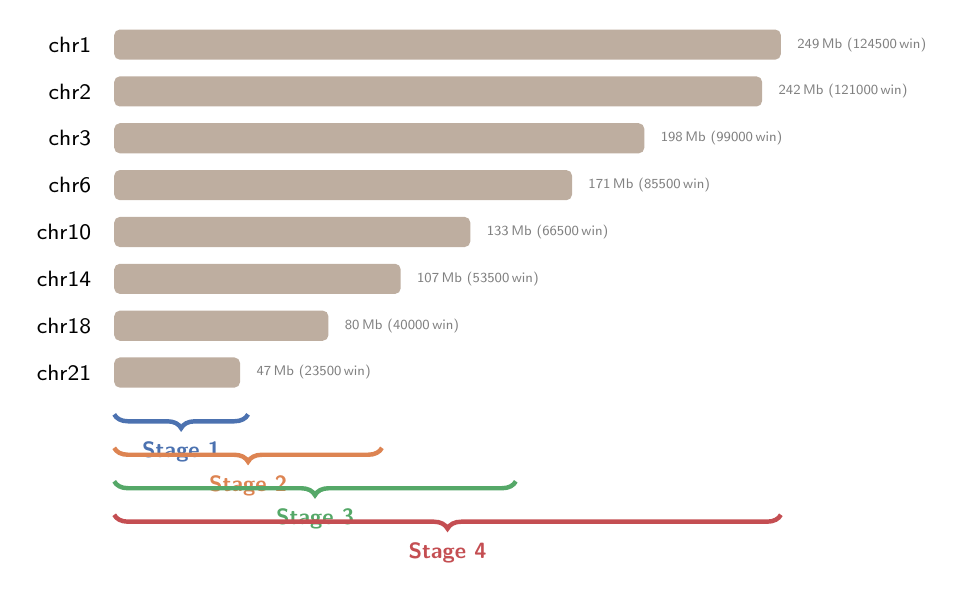
\begin{tikzpicture}[scale=0.85]
  % Draw chromosomes as rounded rectangles with varying lengths
  \foreach \chr/\len/\win/\ypos in {
    1/249/124500/0,
    2/242/121000/-0.7,
    3/198/99000/-1.4,
    6/171/85500/-2.1,
    10/133/66500/-2.8,
    14/107/53500/-3.5,
    18/80/40000/-4.2,
    21/47/23500/-4.9%
  } {
    \pgfmathsetmacro{\w}{\len/25}
    \fill[chrcolor!60, rounded corners=2pt] (0,\ypos) rectangle (\w,\ypos+0.45);
    \node[left, font=\footnotesize\sffamily] at (-0.2,\ypos+0.225) {chr\chr};
    \node[right, font=\tiny\sffamily, gray] at (\w+0.1,\ypos+0.225) {\len\,Mb (\win\,win)};
  }

  % Stage coverage brackets
  \draw[stage1, ultra thick, decorate, decoration={brace, amplitude=5pt, mirror}]
    (0,-5.3) -- (2,-5.3) node[midway, below=6pt, font=\footnotesize\sffamily\bfseries, stage1] {Stage 1};
  \draw[stage2, ultra thick, decorate, decoration={brace, amplitude=5pt, mirror}]
    (0,-5.8) -- (4,-5.8) node[midway, below=6pt, font=\footnotesize\sffamily\bfseries, stage2] {Stage 2};
  \draw[stage3, ultra thick, decorate, decoration={brace, amplitude=5pt, mirror}]
    (0,-6.3) -- (6,-6.3) node[midway, below=6pt, font=\footnotesize\sffamily\bfseries, stage3] {Stage 3};
  \draw[stage4, ultra thick, decorate, decoration={brace, amplitude=5pt, mirror}]
    (0,-6.8) -- (9.96,-6.8) node[midway, below=6pt, font=\footnotesize\sffamily\bfseries, stage4] {Stage 4};
\end{tikzpicture}
\caption{Human chromosome lengths and the sequence lengths covered by each curriculum stage. Stage~4 (250\,Mb) covers the full extent of chr1.}
\label{fig:chromosomes}
\end{figure}

%% =========================================================================
\section{Architecture: Mamba Encoder--Decoder}
%% =========================================================================

The model processes site frequency spectrum (SFS) features computed in non-overlapping 2\,kb windows along the genome. A multi-scale convolutional stem encodes each window independently, then a stack of Mamba layers captures long-range dependencies along the chromosome.

\begin{figure}[h]
\centering
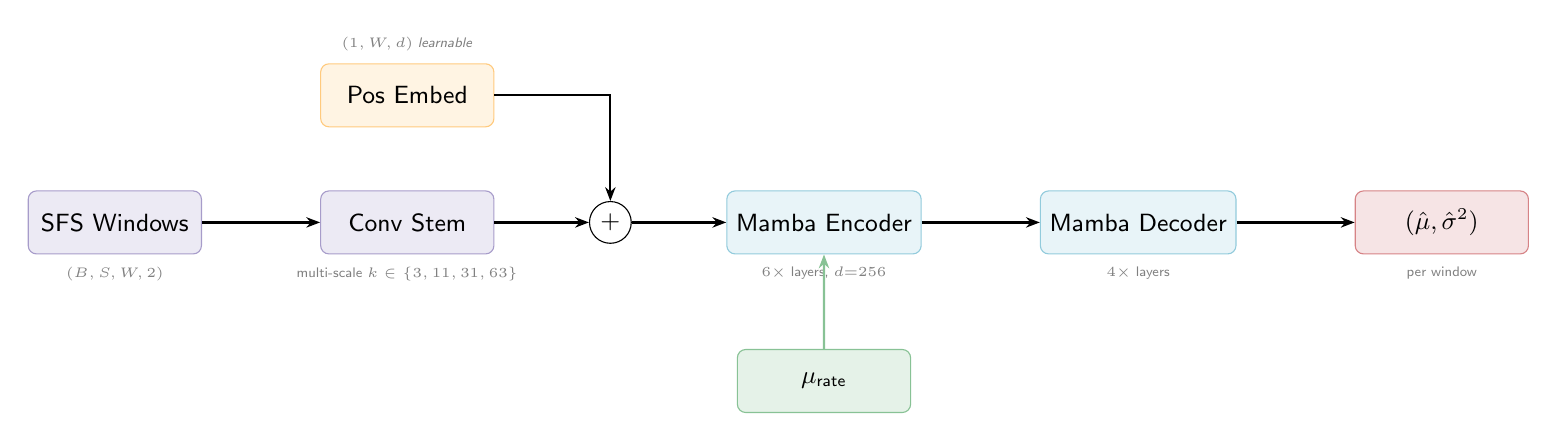
\begin{tikzpicture}[
  block/.style={draw, rounded corners=3pt, minimum height=0.8cm, minimum width=2.2cm, font=\small\sffamily, fill=#1!15, draw=#1!70},
  arrow/.style={-{Stealth[length=5pt]}, thick},
  label/.style={font=\tiny\sffamily, gray},
  scale=0.9
]
  % Input
  \node[block=sfs] (sfs) at (0,0) {SFS Windows};
  \node[label, below=1pt of sfs] {$(B, S, W, 2)$};

  % Stem
  \node[block=sfs, right=1.5cm of sfs] (stem) {Conv Stem};
  \node[label, below=1pt of stem] {multi-scale $k\in\{3,11,31,63\}$};

  % Pos embed
  \node[block=posemb, above=0.8cm of stem] (pos) {Pos Embed};
  \node[label, above=1pt of pos] {$(1, W, d)$ \textit{learnable}};

  % Add
  \node[circle, draw, inner sep=2pt, font=\small, right=1.2cm of stem] (add) {$+$};

  % Encoder
  \node[block=mamba, right=1.2cm of add] (enc) {Mamba Encoder};
  \node[label, below=1pt of enc] {$6\times$ layers, $d{=}256$};

  % Decoder
  \node[block=mamba, right=1.5cm of enc] (dec) {Mamba Decoder};
  \node[label, below=1pt of dec] {$4\times$ layers};

  % Output
  \node[block=stage4, right=1.5cm of dec] (out) {$(\hat\mu, \hat\sigma^2)$};
  \node[label, below=1pt of out] {per window};

  % Arrows
  \draw[arrow] (sfs) -- (stem);
  \draw[arrow] (stem) -- (add);
  \draw[arrow] (pos) -| (add);
  \draw[arrow] (add) -- (enc);
  \draw[arrow] (enc) -- (dec);
  \draw[arrow] (dec) -- (out);

  % Mutation rate conditioning
  \node[block=stage3, below=1.2cm of enc] (mu) {$\mu_{\text{rate}}$};
  \draw[arrow, stage3!70] (mu) -- (enc);
\end{tikzpicture}
\caption{Model architecture. SFS features from each 2\,kb window are encoded by a multi-scale convolutional stem, combined with learnable positional embeddings, then processed by a Mamba encoder--decoder stack. The model outputs a Gaussian $(\mu, \log\sigma^2)$ per window for TMRCA prediction.}
\label{fig:architecture}
\end{figure}

\paragraph{Key property: linear scaling.} Unlike Transformers whose attention is $O(W^2)$, Mamba's selective state space layers are $O(W)$ in sequence length $W$. This makes chromosome-scale sequences (up to 125k windows) tractable with constant per-window cost.

%% =========================================================================
\section{Curriculum Learning Strategy}
%% =========================================================================

We train in four stages of increasing sequence length. Each stage fine-tunes from the previous checkpoint, with the number of training replicates decreasing as simulation cost increases.

\begin{figure}[h]
\centering
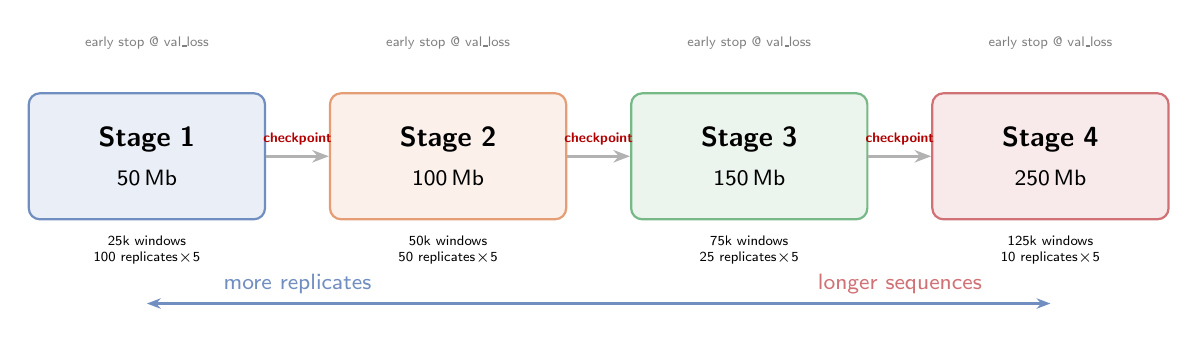
\begin{tikzpicture}[
  stage/.style={draw, rounded corners=4pt, minimum height=1.6cm, minimum width=3.0cm, font=\sffamily, thick, fill=#1!12, draw=#1!80, text width=2.6cm, align=center},
  meta/.style={font=\tiny\sffamily, text width=2.6cm, align=center},
  arrow/.style={-{Stealth[length=6pt]}, very thick, gray!60},
  ckpt/.style={font=\tiny\sffamily\bfseries, red!70!black},
  scale=0.85
]
  % Stage boxes
  \node[stage=stage1] (s1) at (0,0) {\textbf{Stage 1}\\[2pt]\footnotesize 50\,Mb};
  \node[meta, below=2pt of s1] {25k windows\\100 replicates$\times$5};

  \node[stage=stage2] (s2) at (4.5,0) {\textbf{Stage 2}\\[2pt]\footnotesize 100\,Mb};
  \node[meta, below=2pt of s2] {50k windows\\50 replicates$\times$5};

  \node[stage=stage3] (s3) at (9,0) {\textbf{Stage 3}\\[2pt]\footnotesize 150\,Mb};
  \node[meta, below=2pt of s3] {75k windows\\25 replicates$\times$5};

  \node[stage=stage4] (s4) at (13.5,0) {\textbf{Stage 4}\\[2pt]\footnotesize 250\,Mb};
  \node[meta, below=2pt of s4] {125k windows\\10 replicates$\times$5};

  % Arrows with checkpoint labels
  \draw[arrow] (s1) -- (s2) node[midway, above, ckpt] {checkpoint};
  \draw[arrow] (s2) -- (s3) node[midway, above, ckpt] {checkpoint};
  \draw[arrow] (s3) -- (s4) node[midway, above, ckpt] {checkpoint};

  % Early stopping indicators
  \foreach \s in {s1,s2,s3,s4} {
    \node[font=\tiny\sffamily, gray, above=12pt of \s] {early stop @ val\_loss};
  }

  % Training samples arrow
  \draw[{Stealth[length=5pt]}-{Stealth[length=5pt]}, thick, stage1!80]
    (0,-2.2) -- (13.5,-2.2);
  \node[font=\footnotesize\sffamily, stage1!80, above] at (2.25,-2.2) {more replicates};
  \node[font=\footnotesize\sffamily, stage4!80, above] at (11.25,-2.2) {longer sequences};
\end{tikzpicture}
\caption{Curriculum learning pipeline. Each stage trains until early stopping triggers (patience\,=\,20 on validation loss), then the checkpoint is used to initialize the next stage with extended positional embeddings. The trade-off between replicates and sequence length reflects simulation cost.}
\label{fig:curriculum}
\end{figure}

\begin{table}[h]
\centering
\caption{Curriculum stage configuration. All stages use sample sizes $n\in\{10, 25, 50, 100, 200\}$ (``$\times$5''), 2\,kb windows, batch size 4, gradient accumulation 64.}
\label{tab:stages}
\begin{tabular}{@{}lcccccc@{}}
\toprule
Stage & Seq.\ Length & $W$ (windows) & Replicates/size & Preset & Sim Partition & Train Partition \\
\midrule
1 & 50\,Mb  & 25{,}000  & 100 & \texttt{base\_25k}  & genoa (2d) & dgx-b200 (7d) \\
2 & 100\,Mb & 50{,}000  & 50  & \texttt{base\_50k}  & genoa (2d) & dgx-b200 (7d) \\
3 & 150\,Mb & 75{,}000  & 25  & \texttt{base\_75k}  & genoa (4d) & dgx-b200 (7d) \\
4 & 250\,Mb & 125{,}000 & 10  & \texttt{base\_125k} & genoa (4d) & dgx-b200 (7d) \\
\bottomrule
\end{tabular}
\end{table}

%% =========================================================================
\section{Positional Embedding Extension}
%% =========================================================================

The positional embedding is a learnable parameter of shape $(1, W, d)$. At each stage transition, we must extend it to accommodate the larger sequence length. Our approach preserves existing positions and initializes new ones:

\begin{figure}[h]
\centering
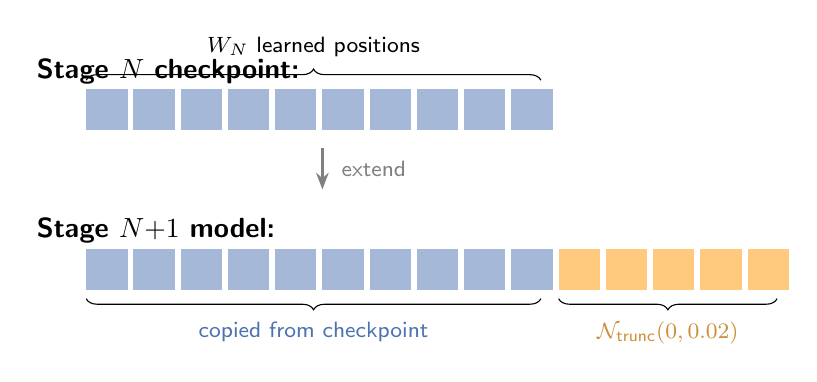
\begin{tikzpicture}[scale=0.75]
  % Stage N embedding
  \node[font=\sffamily\bfseries, anchor=west] at (-1, 2.5) {Stage $N$ checkpoint:};
  \foreach \i in {0,...,9} {
    \fill[stage1!50] (\i*0.8, 1.5) rectangle (\i*0.8+0.7, 2.2);
  }
  \draw[decorate, decoration={brace, amplitude=4pt}] (0,2.35) -- (7.7,2.35)
    node[midway, above=5pt, font=\footnotesize\sffamily] {$W_N$ learned positions};

  % Arrow
  \draw[-{Stealth[length=6pt]}, very thick, gray] (4, 1.2) -- (4, 0.5)
    node[midway, right=3pt, font=\footnotesize\sffamily] {extend};

  % Stage N+1 embedding
  \node[font=\sffamily\bfseries, anchor=west] at (-1, -0.2) {Stage $N{+}1$ model:};
  \foreach \i in {0,...,9} {
    \fill[stage1!50] (\i*0.8, -1.2) rectangle (\i*0.8+0.7, -0.5);
  }
  \foreach \i in {10,...,14} {
    \fill[posemb!70] (\i*0.8, -1.2) rectangle (\i*0.8+0.7, -0.5);
  }
  \draw[decorate, decoration={brace, amplitude=4pt, mirror}] (0,-1.35) -- (7.7,-1.35)
    node[midway, below=5pt, font=\footnotesize\sffamily, stage1] {copied from checkpoint};
  \draw[decorate, decoration={brace, amplitude=4pt, mirror}] (8,-1.35) -- (11.7,-1.35)
    node[midway, below=5pt, font=\footnotesize\sffamily, posemb!80!black] {$\mathcal{N}_{\text{trunc}}(0, 0.02)$};
\end{tikzpicture}
\caption{Positional embedding extension. Existing positions (blue) are preserved exactly from the checkpoint. New positions (orange) are initialized from a truncated normal distribution, matching the original initialization scheme. No interpolation is needed since positions represent fixed 2\,kb genomic intervals.}
\label{fig:posembed}
\end{figure}

This is more principled than interpolation for our setting: each position corresponds to an absolute genomic coordinate at fixed 2\,kb spacing. The model has already learned meaningful representations for positions 1--$W_N$; we simply add new positions $W_N{+}1$ to $W_{N+1}$ with fresh initialization.

%% =========================================================================
\section{Simulation Design}
%% =========================================================================

Training data is generated using \texttt{stdpopsim} with the \texttt{HomSap} species. This provides a natural mixture of demographic histories:

\begin{figure}[h]
\centering
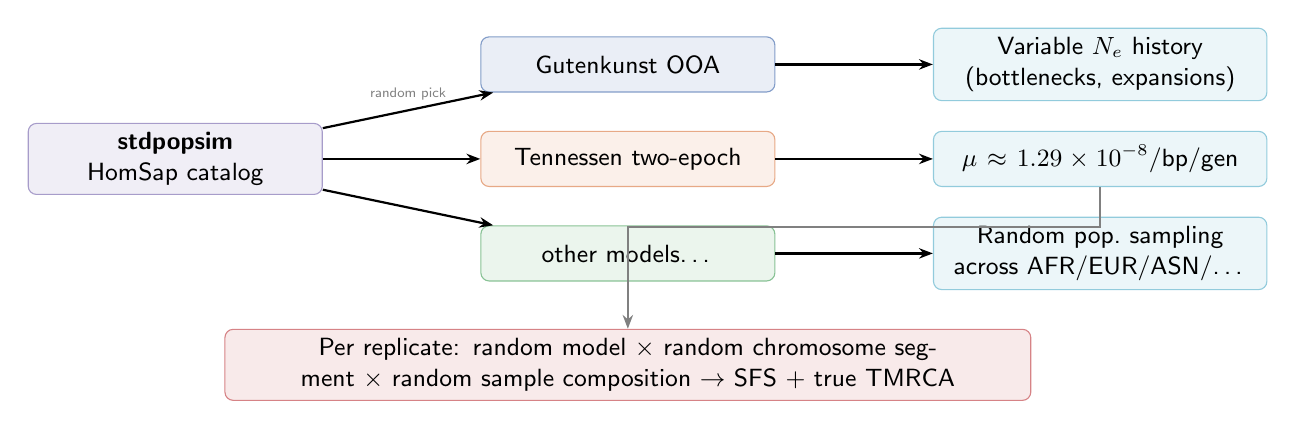
\begin{tikzpicture}[
  box/.style={draw, rounded corners=3pt, minimum height=0.7cm, font=\small\sffamily, fill=#1!12, draw=#1!70, text width=3.5cm, align=center},
  arrow/.style={-{Stealth[length=5pt]}, thick},
  scale=0.85
]
  % stdpopsim
  \node[box=sfs] (std) at (0,0) {\textbf{stdpopsim}\\HomSap catalog};

  % Demographic models
  \node[box=stage1, right=2cm of std, yshift=1.2cm] (m1) {Gutenkunst OOA};
  \node[box=stage2, right=2cm of std, yshift=0.0cm] (m2) {Tennessen two-epoch};
  \node[box=stage3, right=2cm of std, yshift=-1.2cm] (m3) {other models\ldots};

  \draw[arrow] (std) -- (m1) node[midway, above, font=\tiny\sffamily, gray] {random pick};
  \draw[arrow] (std) -- (m2);
  \draw[arrow] (std) -- (m3);

  % Properties
  \node[box=mamba, right=2cm of m2, yshift=1.2cm, text width=4cm] (p1) {Variable $N_e$ history\\(bottlenecks, expansions)};
  \node[box=mamba, right=2cm of m2, yshift=0cm, text width=4cm] (p2) {$\mu \approx 1.29\times10^{-8}$/bp/gen};
  \node[box=mamba, right=2cm of m2, yshift=-1.2cm, text width=4cm] (p3) {Random pop.\ sampling\\across AFR/EUR/ASN/\ldots};

  \draw[arrow] (m1.east) -- (p1.west);
  \draw[arrow] (m2.east) -- (p2.west);
  \draw[arrow] (m3.east) -- (p3.west);

  % SFS output
  \node[box=stage4, below=1.8cm of m2, text width=10cm] (out) {%
    Per replicate: random model $\times$ random chromosome segment $\times$ random sample composition $\to$ SFS + true TMRCA};
  \draw[arrow, gray] (p2.south) -- ++(0,-0.6) -| (out.north);
\end{tikzpicture}
\caption{Simulation design. Each replicate randomly draws a demographic model from the stdpopsim HomSap catalog, a random autosomal segment of the target length, and a random allocation of samples across populations. This produces diverse training data reflecting real human genetic variation.}
\label{fig:simulation}
\end{figure}

%% =========================================================================
\section{Training Configuration}
%% =========================================================================

\begin{figure}[h]
\centering
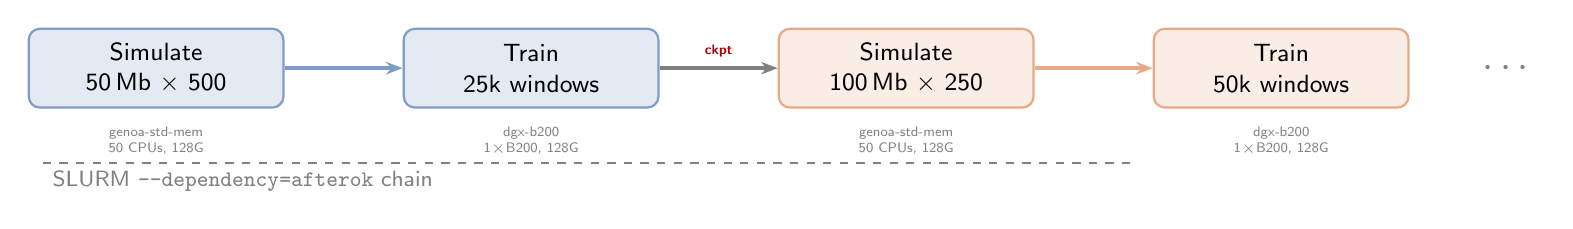
\begin{tikzpicture}[
  proc/.style={draw, rounded corners=4pt, minimum height=1cm, font=\small\sffamily, thick, fill=#1!15, draw=#1!70, text width=3cm, align=center},
  arrow/.style={-{Stealth[length=6pt]}, very thick},
  scale=0.8
]
  % SLURM pipeline
  \node[proc=stage1] (sim1) at (0,0) {Simulate\\50\,Mb $\times$ 500};
  \node[proc=stage1, right=1.5cm of sim1] (train1) {Train\\25k windows};

  \node[proc=stage2, right=1.5cm of train1] (sim2) {Simulate\\100\,Mb $\times$ 250};
  \node[proc=stage2, right=1.5cm of sim2] (train2) {Train\\50k windows};

  \draw[arrow, stage1!70] (sim1) -- (train1);
  \draw[arrow, gray] (train1) -- (sim2) node[midway, above, font=\tiny\sffamily\bfseries, red!70!black] {ckpt};
  \draw[arrow, stage2!70] (sim2) -- (train2);

  % Continue dots
  \node[font=\Large, gray, right=0.8cm of train2] (dots) {$\cdots$};

  % SLURM labels
  \node[font=\tiny\sffamily, gray, below=3pt of sim1, text width=2.5cm, align=center] {genoa-std-mem\\50 CPUs, 128G};
  \node[font=\tiny\sffamily, gray, below=3pt of train1, text width=2.5cm, align=center] {dgx-b200\\1$\times$B200, 128G};
  \node[font=\tiny\sffamily, gray, below=3pt of sim2, text width=2.5cm, align=center] {genoa-std-mem\\50 CPUs, 128G};
  \node[font=\tiny\sffamily, gray, below=3pt of train2, text width=2.5cm, align=center] {dgx-b200\\1$\times$B200, 128G};

  % Dependency chain
  \draw[dashed, gray, thick] (-1.8,-1.5) -- (15.5,-1.5);
  \node[font=\footnotesize\sffamily, gray, anchor=west] at (-1.8,-1.8) {SLURM \texttt{--dependency=afterok} chain};
\end{tikzpicture}
\caption{SLURM execution pipeline. Simulation and training jobs alternate, connected by dependency chains. Each training job produces a checkpoint consumed by the next stage's training job.}
\label{fig:slurm}
\end{figure}

\paragraph{Training hyperparameters.}
\begin{itemize}[nosep]
  \item Batch size: 4 (actual) $\times$ 64 (gradient accumulation) = 256 effective
  \item Learning rate: $3\times10^{-4}$ with cosine decay
  \item Loss: Beta-NLL ($\beta=0.5$) for heteroscedastic TMRCA prediction
  \item Early stopping: patience 20 epochs on validation loss ($\delta_{\min}=10^{-4}$)
  \item Precision: bf16-mixed
  \item Max epochs: 200 (early stopping typically triggers well before)
\end{itemize}

%% =========================================================================
\section{Expected Outcomes}
%% =========================================================================

\begin{figure}[h]
\centering
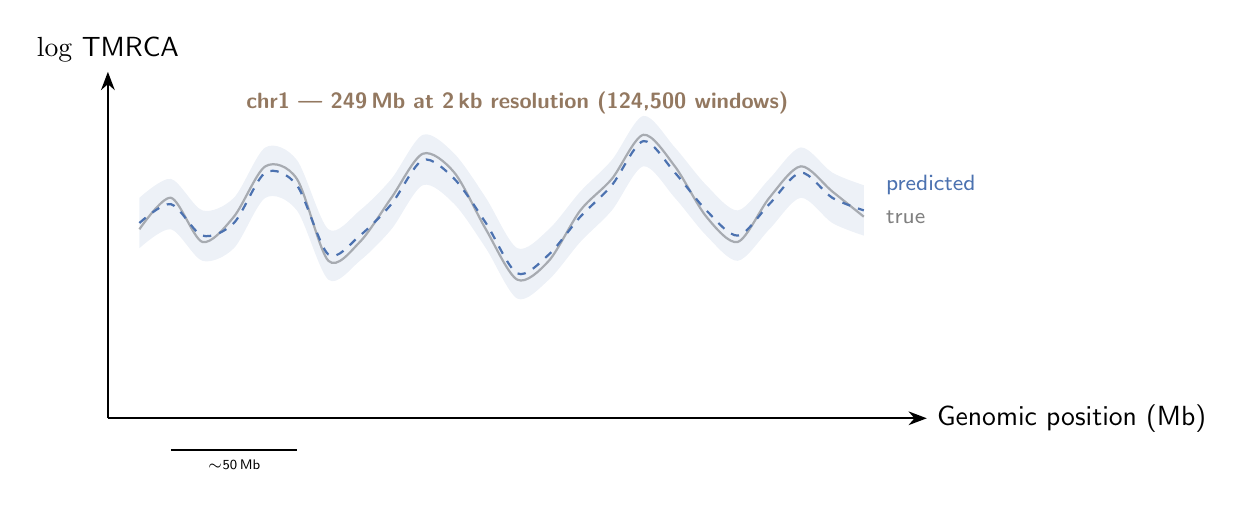
\begin{tikzpicture}[scale=0.8]
  % Axes
  \draw[-{Stealth}, thick] (0,0) -- (13,0) node[right, font=\sffamily] {Genomic position (Mb)};
  \draw[-{Stealth}, thick] (0,0) -- (0,5.5) node[above, font=\sffamily] {$\log$ TMRCA};

  % True signal (wavy line)
  \draw[gray!60, thick] plot[smooth, tension=0.5] coordinates {
    (0.5,3) (1,3.5) (1.5,2.8) (2,3.2) (2.5,4) (3,3.8) (3.5,2.5) (4,2.8)
    (4.5,3.5) (5,4.2) (5.5,3.9) (6,3) (6.5,2.2) (7,2.5) (7.5,3.3) (8,3.8)
    (8.5,4.5) (9,4) (9.5,3.2) (10,2.8) (10.5,3.5) (11,4) (11.5,3.6) (12,3.2)
  };
  \node[font=\footnotesize\sffamily, gray, anchor=west] at (12.2,3.2) {true};

  % Predicted (follows true closely with slight offset)
  \draw[stage1, thick, dashed] plot[smooth, tension=0.5] coordinates {
    (0.5,3.1) (1,3.4) (1.5,2.9) (2,3.1) (2.5,3.9) (3,3.7) (3.5,2.6) (4,2.9)
    (4.5,3.4) (5,4.1) (5.5,3.8) (6,3.1) (6.5,2.3) (7,2.6) (7.5,3.2) (8,3.7)
    (8.5,4.4) (9,3.9) (9.5,3.3) (10,2.9) (10.5,3.4) (11,3.9) (11.5,3.5) (12,3.3)
  };
  \node[font=\footnotesize\sffamily, stage1, anchor=west] at (12.2,3.7) {predicted};

  % Confidence band
  \fill[stage1, opacity=0.1] plot[smooth, tension=0.5] coordinates {
    (0.5,3.5) (1,3.8) (1.5,3.3) (2,3.5) (2.5,4.3) (3,4.1) (3.5,3.0) (4,3.3)
    (4.5,3.8) (5,4.5) (5.5,4.2) (6,3.5) (6.5,2.7) (7,3.0) (7.5,3.6) (8,4.1)
    (8.5,4.8) (9,4.3) (9.5,3.7) (10,3.3) (10.5,3.8) (11,4.3) (11.5,3.9) (12,3.7)
  } -- plot[smooth, tension=0.5] coordinates {
    (12,2.9) (11.5,3.1) (11,3.5) (10.5,3.0) (10,2.5) (9.5,2.9) (9,3.5) (8.5,4.0)
    (8,3.3) (7.5,2.8) (7,2.2) (6.5,1.9) (6,2.7) (5.5,3.4) (5,3.7) (4.5,3.0)
    (4,2.5) (3.5,2.2) (3,3.3) (2.5,3.5) (2,2.7) (1.5,2.5) (1,3.0) (0.5,2.7)
  } -- cycle;

  % Chromosome label
  \node[font=\footnotesize\sffamily\bfseries, chrcolor] at (6.5,5) {chr1 --- 249\,Mb at 2\,kb resolution (124,500 windows)};

  % Scale bar
  \draw[thick] (1,-0.5) -- (3,-0.5);
  \node[font=\tiny\sffamily, below] at (2,-0.5) {$\sim$50\,Mb};
\end{tikzpicture}
\caption{Schematic of expected output: per-window TMRCA prediction with calibrated uncertainty ($\hat\mu \pm 1.96\hat\sigma$) across an entire human chromosome. The model produces both point estimates and confidence intervals, enabling downstream inference of selection, introgression, and demographic history.}
\label{fig:output}
\end{figure}

\paragraph{Applications.} Chromosome-scale TMRCA maps at 2\,kb resolution enable:
\begin{enumerate}[nosep]
  \item Detection of selective sweeps as local TMRCA troughs
  \item Identification of archaic introgression via elevated TMRCA
  \item Fine-scale recombination rate inference from TMRCA transitions
  \item Demographic inference from the genome-wide TMRCA distribution
\end{enumerate}

\noindent The curriculum learning approach makes this feasible without requiring chromosome-scale simulation at full volume, leveraging the Mamba architecture's ability to generalize learned local patterns to longer contexts.

\end{document}
